\chapter{Fundamentação Teórica}


\section{Fundamentação Teórica A}

Nesse exemplo, temos a inserção de figuras no modo basico, que é a figura centralizada e com legenda.

%Exemplo de como inserir figura 

	\begin{figure}[h!]
		\centering
		\Caption{\label{fig:exemplo-1} Lorem ipsum dolor sit amet, consectetur adipiscing elit. Suspendisse commodo lectus et augue elementum varius.}	%legenda%
		\UECEfig{}{
			\fbox{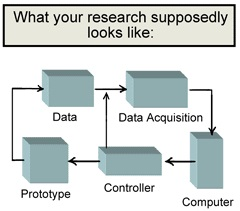
\includegraphics[width=8cm]{figuras/figura-1}}
		}{
			\Fonte{Elaborado pelo autor}
		}	
	\end{figure}
	


\section{Fundamentação Teórica B}

Exemplos de tabelas e figuras.

	\begin{table}[h!]	
		\centering
		\Caption{\label{tab:exemplo-1} Inserir a legenda}		
		\UECEtab{}{
			\begin{tabular}{cll}
				\toprule
				Ranking & Exon Coverage & Splice Site Support \\
				\midrule \midrule
				E1 & Complete coverage by a single transcript & Both splice sites\\
				E2 & Complete coverage by more than a single transcript & Both splice sites\\
				E3 & Partial coverage & Both splice sites\\
				E4 & Partial coverage & One splice site\\
				E5 & Complete or partial coverage & No splice sites\\
				E6 & No coverage & No splice sites\\
				\bottomrule
			\end{tabular}
		}{
		\Fonte{Elaborado pelo autor}
	}
	\end{table}

	\begin{table}[h!]	
		\centering
		\Caption{\label{tab:exemplo-2} Etiam molestie, nulla a egestas aliquet, velit augue congue metus}		
		\UECEtab{}{
			\begin{tabular}{ccll}
				\toprule
				Quisque & pharetra & tempus & vulputate \\
				\midrule \midrule
				E1 & Complete coverage by a single transcript & Both splice sites\\
				E2 & Complete coverage by more than a single transcript & Both splice sites\\
				E3 & Partial coverage & Both splice sites & Both \\
				E4 & Partial coverage & One splice site & Both \\
				E5 & Complete or partial coverage & No splice sites & Both\\
				E6 & No coverage & No splice sites\\
				\bottomrule
			\end{tabular}
		}{
		\Fonte{Elaborado pelo autor}
	}
	\end{table}
	


\section{FUNDAMENTAÇÃO TEÓRICA C }

Exemplo de como inserir equações matematicas. 

\begin{equation}
\forall x \in \mathbf{R}:
\qquad x^{2} \geq 0
\end{equation}


\begin{equation}
x^{2} \geq 0\qquad
\textrm{para todo }x\in\mathbf{R}
\end{equation}

\begin{displaymath}
y=x^{2}\qquad y’=2x\qquad y’’=2
\end{displaymath}
 
\section{FUNDAMENTAÇÃO TEÓRICA D}
Inserindo Figuras lado a lado.
	\begin{figure}[!htb]
	
\begin{minipage}[b]{0.40\linewidth}
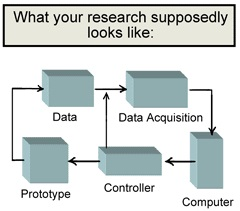
\includegraphics[width=\linewidth]{figuras/figura-1}
\caption{Figura da esquerda}
\label{fig1}
\end{minipage} \hfill
\begin{minipage}[b]{0.40\linewidth}

\includegraphics[width=\linewidth]{figuras/figura-2}
\caption{Figura da direita}
\label{fig2}
\end{minipage}
\end{figure}



\section{FUNDAMENTAÇÃO TEÓRICA E}

Na barra de ferramentas que fica na plataforma Share \LaTeX a esquerda do visor, estará sendo disponibilizado alguns modelos de apostilas para que sirva de ajuda para a edição. E na pasta "README.md" mostra alguns exemplos de inserção de figuras, tabelas, 

\subsection{MONOGRAFIA DE ACORDO COM A ABNT 14724:2011}

Deve apresentar as seguintes informaçoes:

Nome da instituição - corpo de texto, tamanho 12 (Maiúscula).
Nome do autor - corpo de texto, tamanho 12 (Maiúscula). 
Título – corpo de texto, tamanho 12 (Maiúscula); subtítulo (se houver) em letras minúsculas, com exceção da primeira letra de nomes próprios e outros segundo as regras da gramática - corpo de texto, tamanho 12. Local (cidade) e ano de defesa - corpo de texto, 12; 

Lombada é opcional e as informações nela contidas devem ser impressas na seguinte ordem,
conforme NBR 12225 (2004):

Nome do autor, impresso longitudinalmente e legível do alto para o pé da
lombada, de modo a possibilitar a leitura quando o trabalho está no sentido horizontal,
com a face voltada para cima.
Título do trabalho, impresso da mesma forma que o nome do autor. 

\subsection{PARTE INTERNA}

Composta pelos elementos pré-textuais, textuais e pós-textuais.

\subsection{ELEMENTOS PRÉ-TEXTUAIS}
Devem ser apresentados na ordem que segue.

FOLHA DE ROSTO – OBRIGATÓRIO

Apresenta as informações essenciais para a identificação do trabalho na seguinte ordem:
Nome completo do autor – centralizado – tamanho 12 (em maiúscula). 
Título – corpo de texto, tamanho 12 (Maiúscula); subtítulo (se houver) em letras
minúsculas, com exceção da primeira letra de nomes próprios e outros segundo as
regras da gramática - corpo de texto, tamanho 12.
Natureza do trabalho (tese, dissertação, trabalho de conclusão de curso e outros) e
objetivo (aprovação em disciplina, grau pretendido e outros); nome da instituição a
que é submetido; área de concentração - corpo de texto, tamanho 12.
Nome do orientador e se houver o do co-orientador, corpo de texto, tamanho 12.
Local (cidade) da instituição onde deve ser apresentado, corpo de texto, tamanho12.
Ano de depósito do trabalho - corpo de texto, tamanho 12. 

ERRATA - OPCIONAL

FOLHA DE APROVAÇÃO – OBRIGATÓRIO

Elemento obrigatório, colocado logo após a folha de rosto, constitui-se de:

Nome completo do autor.

Título e subtítulo do trabalho (se houver), separados por dois pontos.

Número de volumes (se houver mais de um, deve constar em cada folha de rosto a especificação do respectivo volume).
 Natureza do trabalho (tese, dissertação, trabalho de conclusão de curso e outros) e objetivo (aprovação em disciplina, grau pretendido e outros).
 
 Nome da instituição a que é submetido.
 
 Área de concentração.
 
 Data de aprovação.
 
Nome completo, titulação, afiliação e assinatura dos componentes da banca
examinadora. 

DEDICATÓRIA - OPCIONAL 


AGRADECIMENTOS - OPCIONAL 

NBR 14724, 2005, p. 1

EPÍGRAFE - OPCIONAL

NBR 10520

RESUMO EM PORTUGUÊS E EM LÍNGUA ESTRANGEIRA - OBRIGATÓRIO

ABNT NBR 6028”. (NBR 14724, p. 7)

LISTA DE ILUSTRAÇÕES - OPCIONAL

NBR 14724, 2011, p.8

LISTA DE TABELAS - OPCIONAL 

NBR 14724, 2011, p. 8

LISTA DE ABREVIATURAS E SIGLAS - OPCIONAL 

NBR 14724, 2011, p. 8

LISTA DE SÍMBOLOS - OPCIONAL

NBR 14724, 2011, p. 8

SUMÁRIO - OBRIGATÓRIO

De acordo com a NBR 6027 (2003, p. 2) o título SUMÁRIO deve ser centralizado, escrito em letras maiúsculas e com a mesma tipologia da fonte utilizada para as seções principais.

A subordinação dos itens do sumário deve ser destacada pela apresentação
tipográfica utilizada no texto. 

Os elementos pré-textuais não devem constar no sumário.

Os indicativos das seções que compõem o sumário, se houver, devem ser
alinhados à esquerda, conforme a NBR 6024 (2003, p. 2). 

\subsection{ELEMENTOS TEXTUAIS}

São constituídos de três partes fundamentais: introdução,
desenvolvimento e conclusão intimamente relacionadas como partes de uma estrutura lógica e
harmoniosa. 

INTRODUÇÃO 

NBR 1424, 2005, p. 6

DESENVOLVIMENTO 

Parte principal do texto que contém a exposição ordenada e pormenorizada do assunto.
Divide-se em seções e subseções que variam em função da abordagem do tema e do método. 

CONCLUSÃO 

Parte final do texto, na qual se apresentam as conclusões correspondentes aos objetivos
ou hipóteses. 

ELEMENTOS DE APOIO AO TEXTO: CITAÇÕES E OUTROS (NBR 10520, 2002) 
quanto à forma: literal ou paráfrase;

Tamanho: breve (até três linhas) e longo (com mais de três linhas);

Documento: direta (transcrição fiel da fonte); indireta (transcrição livre da fonte); citação de citação (transcrição direta ou indireta de um texto a cujo conteúdo original não se teve acesso). 

Os outros elementos inseridos no corpo do texto são:

Notas de referência, que indicam fontes consultadas ou remetem a outras partes da obra onde o assunto foi abordado.

Notas de rodapé, que se constituem como indicações, observações ou aditamentos ao texto feitos pelo autor, tradutor ou editor, podendo também aparecer na margem esquerda ou direita da mancha gráfica.

 Notas explicativas, usadas para comentários, esclarecimentos ou explanações, que não possam ser incluídos no texto. 

INDICAÇÃO DAS FONTES DAS CITAÇÕES PELO SISTEMA AUTOR-DATA.

A citação direta de até três linhas pode ser inserida no
próprio parágrafo, entre aspas. A citação direta com mais de três linhas deve aparecer em parágrafo distinto, com recuo de 4 cm da margem esquerda, sem aspas, em espaço simples e com fonte menor que a do texto.

A citação indireta pode ocorrer por paráfrase (aproximadamente do mesmo tamanho do original) e por condensação (quando se faz uma
síntese do texto consultado). A citação de citação deve ser usada apenas na total impossibilidade de acesso ao documento original.

\subsection{ELEMENTOS PÓS-TEXTUAIS}
A ordem dos elementos deve ser apresentada como segue. 

REFERÊNCIAS - OBRIGATÓRIO
NBR 14724, 2011, p. 3, deve ser escrita da forma como esse exemplo:

SOBRENOME DO AUTOR (em maiúsculas, seguido de vírgula), Prenomes (abreviados ou não, sendo apenas as iniciais maiúsculas; é importante respeitar o padrão assumido).

Título
da obra (pode ser em negrito): subtítulo (se houver, precedido por dois pontos, normal).

Tradução (se houver). Edição (se houver, deve ser indicada em algarismo arábico, com ponto e seguido da abreviatura de “edição”).

Local: (após o nome da cidade coloca-se dois pontos) nome da editora (deve ser indicada tal como aparece no documento, abreviando-se os
prenomes e suprimindo a natureza jurídica ou comercial), ano.

Número de páginas

Séries ou coleções (se houver, entre parênteses). 

GLOSSÁRIO - OPCIONAL 

Consiste numa relação de palavras ou de expressões técnicas de uso restrito ou que são pouco conhecidas, utilizadas no texto, acompanhadas das respectivas definições. Deve ser ordenado alfabeticamente.

APÊNDICE(S) – OPCIONAL

NBR 14724, 2011

Exemplos:

APÊNDICE A - Avaliação de desempenho artístico na pré-escola

APÊNDICE B - Avaliação de desempenho artístico na infância 

ANEXO(S) – OPCIONAL

NBR 14724, 2011

ÍNDICE - OPCIONAL

NBR 6034, 2004

\subsection{REGRAS GERAIS DE APRESENTAÇÃO }

Os trabalhos acadêmicos devem ser digitados na cor preta (ficando livre o uso de cores para
as ilustrações), em papel branco ou reciclado, fonte 12 para todo o trabalho, inclusive
capa, excetuando-se citações com mais de três linhas, notas de rodapé, legendas e fontes das
ilustrações e tabelas, que devem ser em tamanho menor e uniforme.

Os elementos pré-textuais devem sempre iniciar no anverso da folha e os textuais e póstextuais
podem ser digitados no anverso e verso das folhas. Para o anverso as margens devem
ser esquerda e superior de 3cm e direita e inferior de 2cm; para o verso, direita e superior de 3
cm e esquerda e inferior de 2 cm.
Usa-se espaço 1,5 entre as linhas nos elementos textuais e espaço simples nas citações com
mais de três linhas, notas de rodapé, referências, legendas e tabelas, natureza do trabalho ou
do projeto na folha de rosto.

As referências ao final do trabalho ou projeto devem ser
separadas entre si por um espaço simples em branco. Os títulos das seções em relação ao
texto que o sucede e os títulos das subseções em relação aos textos que os precede ou sucede
devem ser separados por um espaço 1,5 entre as linhas em branco. 

\subsection{Segundo a NBR 6024:}

a) os títulos das partes (seções) em que se divide o trabalho devem ser precedidos de um
indicativo numérico segundo o sistema de numeração progressiva, sempre alinhados à
esquerda, e começar sempre por um numero inteiro (ex.: 1);

b) devem-se utilizar números arábicos para enumeração das seções/subseções, bem como o
ponto para divisão e consequente subordinação das seções (ex. 1.1);

c) o indicativo de seção precede o título, dele separado por um espaço de um caractere;

d) não deve ser utilizado qualquer sinal (hífen, travessão ou ponto) entre o indicativo
numérico da seção e o seu título; não se usa ponto final em títulos e subtítulos.

e) a apresentação das seções e subseções (títulos e subtítulos) deve ser diferenciada
tipograficamente utilizando recursos como negrito, itálico, grifo, caixa alta, versalete,
dentre outros. A escolha é livre, desde que seja padronizada no trabalho todo.
Recomenda-se que os títulos das seções primárias sejam em maiúsculas. Cada nível de
seção deve seguir sua própria padronização;

f) os títulos sem indicativo numérico (ilustrações, sumário, resumo, referências e outros)
devem ser centralizados na página;
g) no Sumário, os títulos das seções e sua enumeração devem estar na mesma ordem e
grafia do corpo do texto. 

\section{FORMATAÇÃO}

Tamanho do papel: A4 (21,0 cm x 29,7 cm);

Margens: 3cm superior e esquerda, 2 cm inferior e direita.

Fonte: Arial ou Times 

Cor da fonte: preta em todo o trabalho

Tamanho da fonte do corpo do texto: 12 pts

Tamanho da fonte de 10pts para:


Citações longas;
Notas de rodapé;
Legendas;
Paginação;

Espaçamento entre linhas 1,5 para todo corpo do texto e de 1,0 (simples) para:


Citações diretas (mais de 3 linhas);
Notas de rodapé;
Legendas dos elementos especiais (gráficos, figuras, quadros e tabelas)
Referências Bibliográficas
Recuo de primeira linha dos parágrafos: 2 cm

\subsection{PAGINAÇÃO}

A numeração deve aparecer a partir dos elementos “textuais”, ou seja, da introdução até o final do trabalho.
As páginas pré-textuais são contadas, mas não numeradas.
A posição da paginação deve ser à 2cm da borda superior da folha.

\subsection{TÍTULOS E SUBTÍTULOS}

São separados do texto que os precede e sucede por 1 espaço de 1,5; 

A indicação é que o destaque destes elementos é feito utilizando-se negrito, itálico, maiúsculas e sublinhado. 

O alinhamento deve seguir a posição horizontal da 1º letra caso haja mais de 1 linha compondo o título ou subtítulo.

\subsection{INDICATIVO NUMÉRICO}

A numeração dos títulos e subtítulos é feita iniciando-se pela introdução e terminando-se na conclusão. 

A numeração é feita em algarismos arábicos e separadas do texto por um espaço em branco (sem ponto ao final do número).

\subsection{TÍTULOS SEM INDICATIVO NUMÉRICO}

Existem alguns títulos que não recebem numeração e, por esta razão, são centralizados na página. São eles:


Agradecimentos;

Resumo;

Listas (figuras, gráficos, tabelas, quadros);

Sumário;

Referências;

Apêndices e Anexos.

\subsection{CITAÇÕES DIRETAS LONGAS (mais de 3 linhas)}

As citações longas devem ter um recuo de 4 cm da margem esquerda do documento.

Estas citações não recebem aspas e nem itálico (salvo palavras estrangeiras).

Pode-se usar o negrito, explicando-se ao final se “grifo nosso” ou “grifo do autor”.

\subsection{CITAÇÕES DIRETAS CURTAS (até 3 linhas)}

As citações curtas devem ter configuração normal de parágrafo, porém com abertura de aspas no início e final da mesma.

\subsection{INDICATIVO DE AUTORIA NAS CITAÇÕES}

Toda citação, seja ela longa, curta, direta ou indireta, deve ter sua respectiva autoria destacada, sob pena de ser considerada plágio. 

\subsection{FIGURAS, GRÁFICOS, QUADROS E TABELAS}

A legenda de qualquer desses elementos deve aparecer na parte superior das mesmas, precedido pela designação correspondente e respectivo número consecutivo. 

Na parte inferior, indicar a fonte (referência) de onde a mesma foi obtida.

Caso o próprio autor do trabalho tenha “construído” o elemento em questão, citar a fonte como: “do autor”. Consultar orientador sobre o melhor termo a adotar nesta situação.

\subsection{NOTAS DE RODAPÉ}

As notas são separadas do texto por uma linha de 5cm, alinhada à margem esquerda do documento;

Seguem alinhamento padronizado dos caracteres tendo-se por base a posição vertical da primeira letra.

\subsection{REFERÊNCIAS BIBLIOGRÁFICAS}

Devem ser separadas entre si por um espaço simples. Obedecem a normatização NBR 6023.




